\begin{figure}[!htbp]\centering
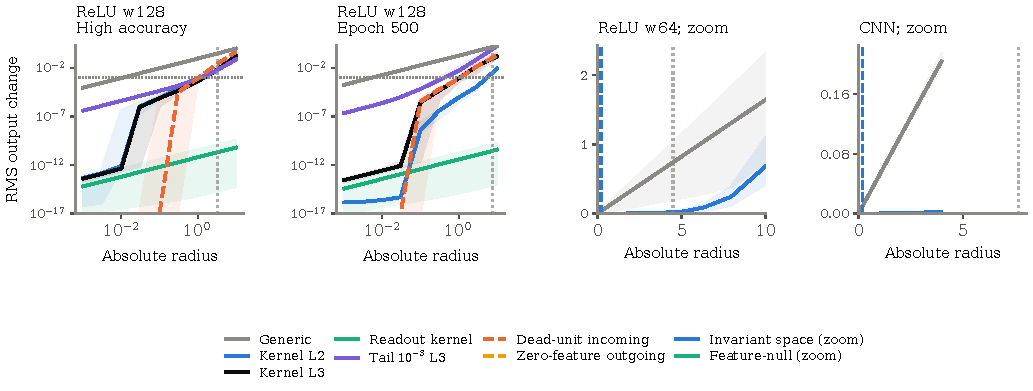
\includegraphics[width=6.195in]{atomic_rays_zoom.pdf}
\caption{Atomic rays and zoomed invariant subspace responses on MNIST. Left pair: width-128 ReLU single-layer kernels, approximate tails and dead-unit controls, with medians of 32 probes per seed and ranges across three seeds; the generic reference edits the whole network. Right pair: seed-0 width-64 MLP and CNN slices, with medians and 10th--90th percentiles over angles; feature-null curves use their own slice axis. These panels use linear axes to resolve visible drift after a first crossing (blue dashed marker). Gray vertical dotted markers give $0.1\|\theta\|_2$; the left panels also mark output visibility at $10^{-3}$. Blue and green retain the invariant-direction and feature-null roles across panels, while the legend distinguishes atomic kernels from multilayer invariant subspaces.}\label{fig:rays-overview}\label{fig:zoom-rays}
\end{figure}
\FloatBarrier
